\documentclass[a4paper,12pt]{article}
\usepackage{amsmath}    % need for subequations
\usepackage{graphicx}   % need for figures
\usepackage{verbatim}   % useful for program listings
\usepackage{color}      % use if color is used in text
\usepackage{subfigure}  % use for side-by-side figures
\usepackage{hyperref}   % use for hypertext links, including those to external documents and URLs
\usepackage{setspace}
\usepackage{natbib}
\usepackage{calligra}
\setlength{\baselineskip}{12.0pt}    % 16 pt usual spacing between lines
\setlength{\topmargin}{-0.5in}
\setlength{\parskip}{3pt plus 2pt}
\setlength{\parindent}{20pt}
\setlength{\oddsidemargin}{0.5cm}
\setlength{\evensidemargin}{0.5cm}
\setlength{\marginparsep}{0.75cm}
\setlength{\marginparwidth}{2.5cm}
\setlength{\marginparpush}{1.0cm}
\setlength{\textwidth}{150mm}
\setlength{\footskip}{0.5cm}
\addtolength{\textheight}{1.2in}

\usepackage{calligra}

\DeclareMathAlphabet{\mathcalligra}{T1}{calligra}{m}{n}
\DeclareFontShape{T1}{calligra}{m}{n}{<->s*[2.2]callig15}{}
\newcommand{\scripty}[1]{\ensuremath{\mathcalligra{#1}}}




% Bibliography and bibfile
\def\aj{AJ}%
          % Astronomical Journal
\def\actaa{Acta Astron.}%
          % Acta Astronomica
\def\araa{ARA\&A}%
          % Annual Review of Astron and Astrophys
\def\apj{ApJ}%
          % Astrophysical Journal
\def\apjl{ApJ}%
          % Astrophysical Journal, Letters
\def\apjs{ApJS}%
          % Astrophysical Journal, Supplement
\def\ao{Appl.~Opt.}%
          % Applied Optics
\def\apss{Ap\&SS}%
          % Astrophysics and Space Science
\def\aap{A\&A}%
          % Astronomy and Astrophysics
\def\aapr{A\&A~Rev.}%
          % Astronomy and Astrophysics Reviews
\def\aaps{A\&AS}%
          % Astronomy and Astrophysics, Supplement
\def\azh{AZh}%
          % Astronomicheskii Zhurnal
\def\baas{BAAS}%
          % Bulletin of the AAS
\def\bac{Bull. astr. Inst. Czechosl.}%
          % Bulletin of the Astronomical Institutes of Czechoslovakia 
\def\caa{Chinese Astron. Astrophys.}%
          % Chinese Astronomy and Astrophysics
\def\cjaa{Chinese J. Astron. Astrophys.}%
          % Chinese Journal of Astronomy and Astrophysics
\def\icarus{Icarus}%
          % Icarus
\def\jcap{J. Cosmology Astropart. Phys.}%
          % Journal of Cosmology and Astroparticle Physics
\def\jrasc{JRASC}%
          % Journal of the RAS of Canada
\def\mnras{MNRAS}%
          % Monthly Notices of the RAS
\def\memras{MmRAS}%
          % Memoirs of the RAS
\def\na{New A}%
          % New Astronomy
\def\nar{New A Rev.}%
          % New Astronomy Review
\def\pasa{PASA}%
          % Publications of the Astron. Soc. of Australia
\def\pra{Phys.~Rev.~A}%
          % Physical Review A: General Physics
\def\prb{Phys.~Rev.~B}%
          % Physical Review B: Solid State
\def\prc{Phys.~Rev.~C}%
          % Physical Review C
\def\prd{Phys.~Rev.~D}%
          % Physical Review D
\def\pre{Phys.~Rev.~E}%
          % Physical Review E
\def\prl{Phys.~Rev.~Lett.}%
          % Physical Review Letters
\def\pasp{PASP}%
          % Publications of the ASP
\def\pasj{PASJ}%
          % Publications of the ASJ
\def\qjras{QJRAS}%
          % Quarterly Journal of the RAS
\def\rmxaa{Rev. Mexicana Astron. Astrofis.}%
          % Revista Mexicana de Astronomia y Astrofisica
\def\skytel{S\&T}%
          % Sky and Telescope
\def\solphys{Sol.~Phys.}%
          % Solar Physics
\def\sovast{Soviet~Ast.}%
          % Soviet Astronomy
\def\ssr{Space~Sci.~Rev.}%
          % Space Science Reviews
\def\zap{ZAp}%
          % Zeitschrift fuer Astrophysik
\def\nat{Nature}%
          % Nature
\def\iaucirc{IAU~Circ.}%
          % IAU Cirulars
\def\aplett{Astrophys.~Lett.}%
          % Astrophysics Letters
\def\apspr{Astrophys.~Space~Phys.~Res.}%
          % Astrophysics Space Physics Research
\def\bain{Bull.~Astron.~Inst.~Netherlands}%
          % Bulletin Astronomical Institute of the Netherlands
\def\fcp{Fund.~Cosmic~Phys.}%
          % Fundamental Cosmic Physics
\def\gca{Geochim.~Cosmochim.~Acta}%
          % Geochimica Cosmochimica Acta
\def\grl{Geophys.~Res.~Lett.}%
          % Geophysics Research Letters
\def\jcp{J.~Chem.~Phys.}%
          % Journal of Chemical Physics
\def\jgr{J.~Geophys.~Res.}%
          % Journal of Geophysics Research
\def\jqsrt{J.~Quant.~Spec.~Radiat.~Transf.}%
          % Journal of Quantitiative Spectroscopy and Radiative Trasfer
\def\memsai{Mem.~Soc.~Astron.~Italiana}%
          % Mem. Societa Astronomica Italiana
\def\nphysa{Nucl.~Phys.~A}%
          % Nuclear Physics A
\def\physrep{Phys.~Rep.}%
          % Physics Reports
\def\physscr{Phys.~Scr}%
          % Physica Scripta
\def\planss{Planet.~Space~Sci.}%
          % Planetary Space Science
\def\procspie{Proc.~SPIE}%
          % Proceedings of the SPIE
          
          
\newcommand{\adv}{    {\it Advances in Space Research}}
\newcommand{\annG}{   {\it Annales Geophysicae}}
\newcommand{\aap}{    {\it Astronomy \& Astrophysics}}
\newcommand{\aaps}{   {\it Astronomy \& Astrophysics Supplemental}}
\newcommand{\aapr}{   {\it Astronomy \& Astrophysics Review}}
\newcommand{\ag}{     {\it Ann. Geophys.}}
\newcommand{\aj}{     {\it Astronomical Journal}}
\newcommand{\apj}{    {\it Astrophysical Journal}}
\newcommand{\apjs}{    {\it Astrophysical Journal Supplemental Series}}
\newcommand{\apjl}{   {\it Astrophysical Journal Letters}}
\newcommand{\apss}{   {\it Astrophysics \& Space Science}}
\newcommand{\cjaa}{   {\it Chinese Journal Astronomy \& Astrophysics}}
\newcommand{\gafd}{   {\it Geophysical and Astrophysical Fluid Dynamics}}
\newcommand{\grl}{    {\it Geophysical Research Letters}}
\newcommand{\ijga}{   {\it International Journal of Geomagnetism and Aeronomy}}
\newcommand{\jastp}{  {\it Journal of Atmospheric and Solar-Terrestrial Physics}}
\newcommand{\jgr}{    {\it Journal of Geophysical Research}}
\newcommand{\mnras}{  {\it Monthly Notices of the Royal Astronomical Society}}
\newcommand{\nat}{    {\it Nature}}
\newcommand{\pasp}{   {\it Publications of the Astronomical Society of the Pacific}}
\newcommand{\pasj}{   {\it Publications of the Astronomical Society of Japan}}
\newcommand{\pra}{    {\it Physical Review A}}
\newcommand{\pre}{    {\it Physical Review E}}
\newcommand{\solphys}{{\it Solar Physics}}
\newcommand{\sovast}{ {\it Soviet Astronomy}}
\newcommand{\ssr}{    {\it Space Science Reviews}}
\newcommand{\araa}{  {\it Annual Review of Astronomy \& Astrophysics}}
\newcommand{\memsai}{ {\it Memorie della Societa Astronomia Italiana}}
\newcommand{\zap}{ {\it Zeitschrift fur Astrophysik}}
\newcommand{\bain}{ {\it Bulletin of the Astronomical Institutes of the Netherlands}}
\newcommand{\planss}{ {\it Planet.~Space~Sci.}}%


\begin{document}

\begin{titlepage}
   \vspace*{\stretch{1.0}}
   \begin{center}
      \Large\textbf{A Bibliography of Stellar Magnetic Flux Tube Models}\\
      \large\textit{Lauren Mc Keown}
   \end{center}
   \vspace*{\stretch{2.0}}
\end{titlepage}


\section{Introduction}

The magnetic influence evidenced in sunspots and active regions of the Solar surface is thought to originate from a strong toroidal magnetic field stemming from the convection zone of the Sun. Magnetic flux tubes are magnetic field concentrations near the surface of the Sun and can explain the mechanism by which magnetic flux may be transported through the convection zone into the Solar atmosphere.\citep{people.hao} My project will focus on how this behaviour may apply to the giants also. 

Given the observed well - defined order of Solar active regions, it makes sense that the tubes maintain reasonable cohesion. Magnetic reconnection on both small and large scales can help to explain the phenomena of surface brightenings and violent outbursts such as CME's and Solar flares, respectively. \citep{Priest2000} This behaviour is important to consider when investigating stellar mass loss among the giants. 

Different computational and mathematical approaches to modelling the flux tube network on the stellar surface have been employed throughout the years - many basic, and others supported strongly by observable evidence. As a first project, I intend to trace these methods back to the beginning and map the mathematical transitions - noting the advances and steps forward taken with each one. From this, I intend to provide a comprehensive basis upon which to be referred back to during my own computational modelling. This bibliography will take the form of subsections defining each approach I find to be significant. I will also provide short descriptions of each method, noting marked techniques evidenced in each.

\section{Important Concepts}

\subsection{Maxwell's Equations}

Maxwell's Equations are the fundamental relations regarding the structure of magnetic flux tubes. Hence, it is useful to go back to the roots of these equations and derive them as follows:

\subsubsection{Maxwell's First Equation (Gauss's Law)}

If we consider a point charge q at the origin of a sphere, we can consider the concept of an electric field, which is a measure of capability to exert a force on the electric charge under inspection. This is expressed by $E=\frac{q}{4\pi\varepsilon_o r^2}\hat{r}$.

Electric flux is known as the measure of the amount of field lines passing through a particular surface S; $d\phi_E=EdAcos\theta$, where $\theta$ represents the angle the field makes with the normal vector to this particular area or object. So when $\theta=90\,^{\circ}$, we have no electric flux. In other words, when the object placed in the field is parallel to the field, we expect zero flux, because the angle between the normal to this area and the electric field lines is $\theta=90\,^{\circ}$ and hence $cos\theta$ and subsequently $d\phi_E$ equates to zero. In contrast, when the object is placed exactly perpendicular to the field lines, we achieve maximum flux. 

If we integrate over the above expression for electric flux passing through an area dA on a sphere, we yield:

\[\phi_E=\int\limits_S E.dA\]



Quantitatively, in the case of a point charge q at the origin, the flux of electric field E through a sphere of radius r is:

\[\oint E.dA = \int \frac{q}{4\pi\varepsilon_o r^2}\hat{r}.(r^2sin\theta d \theta d\phi\hat{r})=\frac{q}{\varepsilon_o}\]


Note that the $r^2$ terms cancel; as the surface area increases as $r^2$, the field goes \emph{down} as $\frac{1}{r^2}$, and so the product is constant. When we consider the \emph{total} flux for a bunch of charges scattered about, we use a (vector) summation of the individual fields $E=\sum\limits_{i=1}^n E_i$. The flux though the surface that encloses all of these individual fields is then:

\[\oint E.dA=\sum\limits_{i=1}^n(\oint E_i.dA)=\sum\limits_{i=1}^n(\frac{q_i}{\varepsilon_o})\]

Hence, for any closed surface:

\[\oint\limits_S E.dA=\frac{Q_e_n_c}{\varepsilon_o}\]

Where $Q_e_n_c$ is the total charge enclosed within the surface. This is Gauss's Law, the first of Maxwell's Equations. The essence of this relation is that; due to the cancellation of the $r^2$ terms, the total flux of E depends on the \emph{charge enclosed} and not on the surface chosen.

If we wish to express Gauss's Law in the form of a \emph{differential} equation, we apply the divergence theorem:

\[\oint\limits_S E.dA=\int\limits_\nu(\nabla.E)d\tau\]

Rewriting $Q_e_n_c$ in terms of the charge density $\rho$ we have:

\[Q_e_n_c=\int\limits_\nu \rho d\tau\]

So by subbing this in, Gauss's Law becomes:

\[\int\limits_\nu (\nabla.E)d\tau=\int\limits_\nu(\frac{\rho}{\varepsilon_o})d\tau\]

And since this holds for \emph{any} volume, the integrands must be equal:

\[\nabla.E=\frac{\rho}{\varepsilon_o}\]

This is the differential form of Gauss's Law. It has an advantage in the sense that it is tidier. However, the integral form accommodates point, line and surface charges more naturally. Note that symmetry is crucial to ease - of - use of this law in dropping the dot product and taking $\mid E \mid$ out of the integral. Note also - Gauss's Law tells us that if we have a charge spread on a sphere, the electric field strength on the surface will be the same as if we had all charge concentrated at the centre of the sphere.


\subsubsection{Maxwell's 2nd Equation (No Magnetic Monopoles)}

First, we define our vector notation. The location of a point in 3D can be described by listing its Cartesian coordinates (x,y,z). The vector to that point from the origin is the \emph{position vector}:

\[\textbf{r}\equiv x\mathbf{\hat{x}}+y\mathbf{\hat{y}}+z\mathbf{\hat{z}}\]

We denote its magnitude (the distace from the origin) by:
\[r=\sqrt{x^2+y^2+z^2}\]

The unit vector pointing radially outward is:

\[\mathbf{\hat{r}}=\frac{\textbf{r}}{r}=\frac{x\mathbf{\hat{x}}+y\mathbf{\hat{y}}+z\mathbf{\hat{z}}}{\sqrt{x^2+y^2+z^2}}\]

The infinitesimal displacement vector, from (x,y,z) to (x+dx,y+dy,z+dz) is:

\[d\mathbf{l}=dx\mathbf{\hat{x}}+dy\mathbf{\hat{y}}+dz\mathbf{\hat{z}}\]

We could call this d\textbf{r}, since that is what it is, but it is useful to keep a special letter for \emph{infinitesimal} displacements.

The source point (where the charge is located) is denoted by \textbf{r'}. The field point (at which we calculate the electric or magnetic field), is denoted by \textbf{r}. The \emph{separation vector} from the source point to the field point is denoted by $\mathbf{R}$.

\[\mathbf{R} \equiv \mathbf{r}-\mathbf{r'}\]

Its magnitude is:

\[R=\mid\mathbf{r}-\mathbf{r'}\mid\]

And a unit vector in the direction from \textbf{r'} to \textbf{r} is:

\[\mathbf{\hat{R}}=\frac{\mathbf{R}}{R}=\frac{\mathbf{r}-\mathbf{r'}}{\mid\mathbf{r}-\mathbf{r'}\mid}\]

In Cartesian coordinates:

\[\mathbf{R}=(x-x')\mathbf{\hat{x}}+(y-y')\mathbf{\hat{y}}+(z-z')\mathbf{\hat{z}}

\[R=\sqrt{(x-x')^2+(y-y')^2+(z-z')^2}\]

\[\hat{R}=\frac{(x-x')\mathbf{\hat{x}}+(y-y')\mathbf{\hat{y}}+(z-z')\mathbf{\hat{z}}}{\sqrt{(x-x')^2+(y-y')^2+(z-z')^2}}\]

Now we can begin with the Biot - Savart Law for the general case of a volume current;


\[B(r)=\frac{\mu_o}{4\pi}\int\ \frac{J(r')\times \hat{R}}{R^2}d\tau'\]

Which gives the magnetic field at a point $r = (x,y,z)$ in terms of an integral over the current distribution \textbf{J}(x',y',z'). Here \textbf{B} is a function of (x,y,z) and \textbf{J} is a function of (x',y',z'). 

\[R=(x-x')\mathbf{\hat{x}}+(y-y')\mathbf{\hat{y}}+(z-z')\mathbf{\hat{z}}\]
\[d\tau'=dx'dy'dz'\]

We integrate over the \emph{primed} coordinates; we take the divergence and curl with respect to the \emph{unprimed} coordinates. Now we apply the divergence to the Biot - Savart Law mentioned above:

\[\nabla \cdot B=\frac{\mu_o}{4\pi}\int \nabla \cdot (J\times \frac{\hat{R}}{R^2})d\tau'\]

Working on the right hand side and using the product rule:

\[\nabla \cdot(\mathbf{J}\times \frac{\mathbf{\hat{R}}}{R^2})={\frac{\mathbf{\hat{R}}}{R^2} \cdot (\nabla\times \mathbf{J})-\mathbf{J} \cdot (\nabla\times\frac{\mathbf{\hat{R}}}{R^2})\]

But $\nabla\times\textbf{J}=0$ because \textbf{J} doesnt depend on the unprimed variables (x,y,z), and $\nabla\times(\frac{\hat{R}}{R^2})=0$ (geometrically, because the curl of $r^n\hat{r}=0$), so by combining these:

\[\nabla \cdot B=0\]

The divergence of the magnetic field is zero. This is similar in effect to the concept of +Q and -Q cancelling each other out in the case of electric charges. Maxwell's 2nd Equation is the magnetic form of Gauss's Law and indicates that there are no point sources of magnetic field. Hence, we can never have an isolated magnetic pole or monopole; the North and South poles of a magnet are always in co - existence. 


\subsubsection{Maxwell's 3rd Equation (Faraday's Law)}



We consider a plain coil of wire and move a magnet in and out of this coil. We know from experiment that current will flow in the loop when the magnet is moving. This is an induced current due and proportional to a changing magnetic field as there exists an induced emf $\epsilon$ causing current I to flow. Similarly, if we move a coil of wire relative to a \emph{stationary magnet}, we again observe a current and hence an induced emf. Faraday deduced that \emph{a changing magnetic field induces an electic field}. It is this induced electric field that is accountable for the induced emf. If this emf is equal to the rate of change of flux,

\[\epsilon=\oint \textbf{E} \cdot d \textbf{l}=\frac{-d \Phi}{dt}\]

then E relates to the change in B by the following:

\[\oint \textbf{E} \cdot dl=-\int \frac{\delta \textbf{B}}{\delta t} \cdot d \textbf{a}\]

This is Faraday's Law, in integral form. It is converted to differential form using Stoke's theorem:

\[\nabla \times \textbf{E}=-\frac{\delta \textbf{B}}{\delta t}\]

Note that Faraday's Law reduces to the old rule $\oint \textbf{E} \cdot d \textbf{l}=0$ (or $\nabla \times \textbf{E}=0$) in the static case where B is constant and $\frac{\delta B}{\delta t}=0$, as it should. From this law, we find the Universal Flux Rule, which states that whenever and for whatever reason the magnetic flux in a loop changes, an emf $\epsilon=\frac{-d \Phi}{dt}$ will appear in the loop. In order to understand the \emph{direction} of the induced current, we use Lenz's Law:

\textbf{Nature abhors a change in flux}

The induced current will flow in such a diection that the flux \emph{it} produces will cancel out the change. For example, if we move a bar magnet through a loop to the left, the flux will increase in the left direction and hence the loop will want to create an opposing flux to the right. Hence, the induced current will flow clockwise. The same effect occurs as the magnet leaves the loop - the loop will want to restore the flux and current will suitably flow counterclockwise.  



\subsubsection{Maxwell's 4th Equation (Amendment to Amp\`{e}re's Law)}

If we apply the curl to the Biot - Savart law, we get:

\[\nabla \cdot \mathbf{B}=\frac{\mu_o}{4\pi}\int \nabla\times(\mathbf{J}\times\frac{\mathbf{\hat{R}}}{R^2})d\tau'\]

Expanding the integrand using the product rule appropriate to this relation, we get:

\[\nabla\times(\mathbf{J}\times\frac{\mathbf{\hat{R}}}{R^2})-(\mathbf{J} \cdot \nabla)\frac{\mathbf{\hat{R}}}{R^2}\]

We have dropped terms containing derivatives of \textbf{J}, because \textbf{J} does not depend on (x,y,z). The second term integrates to zero because we are integrating over the volume that appears in the Biot - Savart Law; one which is large enough to contain all of the current.On the \emph{boundary} the current is zero, so the resulting surface integral goes to zero. Left with the first term, we have:

\[\nabla \cdot (\frac{\mathbf{\hat{R}}}{R^2})=4\pi\delta^3(\mathbf{R})\]

And hence;

\[\nabla \times B=\frac{\mu_o}{4\pi}\int\mathbf{J(r')}4\pi\delta^3(\mathbf{r}-\mathbf{r'})d\tau'=\mu_o\mathbf{J(r)}\]

This is the differential form of Amp\`{e}re's law. We can convert it to integral form by using Stoke's theorem:

\[\int(\nabla \times \mathbf{B}) \cdot d \mathbf{A}=\oint B \cdot d \mathbf{l}=\mu_o \int \mathbf{J} \cdot d \mathbf{A}\]

$\mathbf{J} \cdot d\mathbf{A}$ is the total current passing though the surface, which we call $I_e_n_c$ (the current enclosed by the Amperian loop). Therefore;

\[\oint \mathbf{B} \cdot d\mathbf{l}=\mu_oI_e_n_c\]

This is the integral version of Amp\`{e}re's law and is a generalisation to arbitrary \emph{steady} currents. Note that this equation has a sign ambiguity in the sense that we may be unsure of what \emph{way} to go around the loop and which \emph{direction} through the surface corresponds to a ``positive current". The resolution to this is the right hand rule - if the fingers of one's right hand indicate the direction of integration around the boundary, then one's thumb indicates the direction of a positive current. In particular, for currents with appropriate symmetry, Amp\`{e}re's law in its integral form provides a greatly efficient means for calculating the magnetic field.
 
We shall see now how Maxwell altered this law to allow for the \emph{displacement current}.

Maxwell noticed an inconsistency in his formulae. The divergence of a curl should always be zero. This works for Faraday's Law:

\[\nabla \cdot (\nabla \times E)=\nabla \cdot (-\frac{\delta B}{\delta t})=-\frac{\delta}{\delta t}(\nabla \cdot B)\]

This works because Maxwell's Second Law on the right had side indicates that the divergence of a magnetic field is always zero. However, when we perform the same operation on Amp\`{e}re's Law, we do not yield the same result.

\[\nabla \cdot (\nabla \times B)=\mu_o(\nabla \cdot J)\]

The left hand side must be zero by virtue of the rule stating the divergece of a curl is always zero. However, the right hand side is not zero in general. In the case of \emph{steady} currents, the divegence of J is zero. However, for situations beyond magnetostatics, this case does not hold true. The following situation helps to show why the original version of Amp\`{e}re's law was not sufficient for all cases. We take the integral form of Amp\`{e}re's law:

\[\oint B \cdot dl=\mu_oI_e_n_c\]

We consider a situation where we are charging up a capacitor. We wish to apply Amp\`{e}re's Law to a Amp\`{e}rian loop.$I_e_n_c$ is the total current passing through the loop, or the current piercing the surface that has the loop as its boundary. In our case, the simplest surface lies in the plane of the loop (the wire punctures this surface). Therefore, $I_e_n_c=I$. However, if we construct a balloon - shaped surface encasing one of the plates of the capacitor, we get that $I_e_n_c=0$, as the current does not pierce the surface of the balloon shape. We never faced this problem in magnetostatics because the conflict only arises when charge is piling up somewhere. Note that this flaw in Amp\`{e}re's Law is merely theoretical. Maxwell fixed it as follows:

We take the right hand side of the middle equation above, and apply the continuity equation to it:

\[\nabla \cdot J=-\frac{\delta \rho}{\delta t}=-\frac{\delta}{\delta t}(\varepsilon_o \nabla \cdot E)=-\nabla \cdot (\varepsilon_o \frac{\delta E}{\delta t})\]

We then kill off the extra divergence and add this to J in Amp\`{e}re's Law to get:

\[(\nabla \times B)=\mu_o J +\mu_o \varepsilon_o(\frac{\delta E}{\delta t})\]

The extra term changes nothing when we are considering \emph{magnetostatics}. This is when E is constant and hence $\frac{\delta E}{\delta t}$ amounts to zero. However, the new term has a critical role to play in electromagnetic wave propagation and is known as the \emph{displacement current}. Maxwell's term also tells us that just as a changing magnetic field induces an electric field (Faraday's Law), so too does a changing electric field induce a magnetic field. 




\DeclareGraphicsExtensions{.pdf,.png,.jpg}

%\begin{figure}

%\includegraphics[width=5cm,height=5cm]{hello.ps}

%\end{figure}




\section{Important Flux Tube Papers}

\subsection{Earliest Paper Found so Far: "The Formation of Sunspots from the Solar Toroidal Field"} \citep{parker}

\subsection{Paper on Flux Tube Waves: "An Approximate Flow Equation for Geomagnetic Flux Tubes and its Application to Polar Substorms"}\citep{Atkinson}


\bibliographystyle{plainnat.bst}
\bibliography{mybib}
\end{document}
